
\documentclass[submit]{harvardml}

% Put in your full name and email address.
\name{David Hughes}
\email{davidralphhughes@college.harvard.edu}

% List any people you worked with.
\collaborators{%
    Alexander Munoz
}

% You don't need to change these.
\course{CS181-S18}
\assignment{Assignment \#3}
\duedate{11:59pm March 23, 2018}

\usepackage[OT1]{fontenc}
\usepackage[colorlinks,citecolor=blue,urlcolor=blue]{hyperref}
\usepackage[pdftex]{graphicx}
\usepackage{subfig}
\usepackage{fullpage}
\usepackage{amsmath}
\usepackage{amssymb}
\usepackage{color}
\usepackage{todonotes}
\usepackage{listings}
\usepackage{common}
\usepackage{bm}

\usepackage[mmddyyyy,hhmmss]{datetime}

\definecolor{verbgray}{gray}{0.9}

\lstnewenvironment{csv}{%
  \lstset{backgroundcolor=\color{verbgray},
  frame=single,
  framerule=0pt,
  basicstyle=\ttfamily,
  columns=fullflexible}}{}

\begin{document}
\begin{center}
{\Large Homework 3: Max-Margin and SVM}\\
\end{center}
\subsection*{Introduction}

This homework assignment will have you work with max-margin methods
and SVM classification. The aim of the assignment is (1) to further
develop your geometrical intuition behind margin-based classification
and decision boundaries, (2) to have you implement a basic Kernel-based
classifier and get some experience in implementing a model/algorithm
from an academic paper in the field, and (3) to have you reflect on the
ethics lecture and to address the scenario discussed in class
in more depth by considering the labor market dynamically.

There is a mathematical component and a programming component to this
homework.  Please submit your PDF and Python files to Canvas, and push
all of your work to your GitHub repository. If a question requires you
to make any plots, like Problem 3, please include those in the
writeup.

\newpage
%%%%%%%%%%%%%%%%%%%%%%%%%%%%%%%%%%%%%%%%%%%%%
% Problem 1
%%%%%%%%%%%%%%%%%%%%%%%%%%%%%%%%%%%%%%%%%%%%%
\begin{problem}[Fitting an SVM by hand, 7pts]
  For this problem you will solve an SVM without the help of a
  computer, relying instead on principled rules and properties of
  these classifiers.

Consider a dataset with the following 7 data points each with $x \in \reals$ : \[\{(x_i, y_i)\}_i =\{(-3
, +1 ), (-2 , +1 ) , (-1,  -1 ), (0, -1), ( 1 , -1 ), ( 2 , +1 ), ( 3 , +1 )\}\] Consider
mapping these points to $2$ dimensions using the feature vector $\bphi(x) =  (x, x^2)$. The hard margin classifier training problem is:
%
\begin{align}
  &\min_{\mathbf{w}, w_0} \|\mathbf{w}\|_2^2 \label{eq:dcp} \\
  \quad \text{s.t.} \quad & y_i(\mathbf{w}^\top \bphi(x_i) + w_0) \geq 1,~\forall i \in \{1,\ldots, n\}\notag
\end{align}

The exercise has been broken down into a series of questions, each
providing a part of the solution. Make sure to follow the logical structure of
the exercise when composing your answer and to justify each step.

\begin{enumerate}
\item Plot the training data in $\reals^2$ and draw the decision boundary
of the max margin classifer.
%
\item  What is the value of the margin achieved by the optimal
decision boundary?
%
\item What is a vector that is orthogonal to the decision boundary?

%
\item Considering discriminant $h(\bphi(x);\boldw,w_0)=\boldw^\top\bphi(x) +w_0$,
give an expression for {\em all possible} $(\boldw,w_0)$ that define
the optimal decision boundary. Justify your answer.

  \item Consider now the training problem~\eqref{eq:dcp}. Using
your answers so far, what particular solution
to $\boldw$ will be optimal for this optimization
problem?

  \item Now solve for
the corresponding value of $w_0$, using your general expression
from part~(4.) for the optimal decision boundary.
Write down the discriminant
function $h(\bphi(x);\boldw,w_0)$.


\item What are the support
vectors of the classifier?
 Confirm that the solution in part~(6.) makes the constraints in~\eqref{eq:dcp} binding
for support vectors.

\end{enumerate}

\end{problem}
\subsection*{Solution}

\begin{enumerate}
    \item
        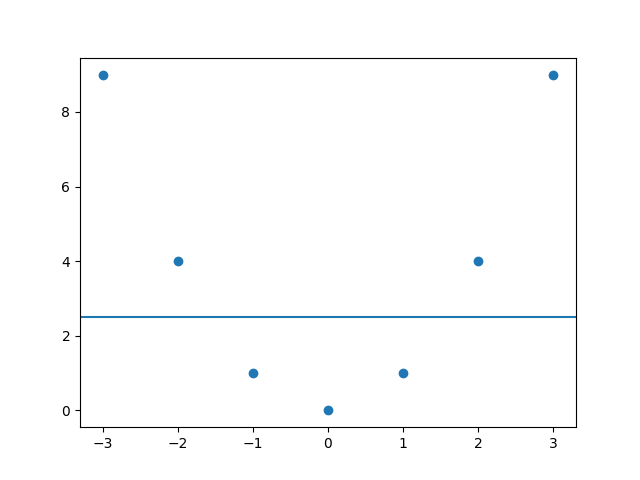
\includegraphics[scale=.5]{prob1.png}
    \item
        r = 1.5
    \item
        $<0,1>$ is orthogonal
    \item
        $\forall i : h(\phi(x))y_i \ge 1$ \\
        This is any $\vec{w}$ that satisfies the hard margin constraint is a
        linear separator \\ \\
        So for our data: \\
        $-3w_1 + 9w_2 + w_0 \ge 1$ \\
        $-2w_1 + 4w_2 + w_0 \ge 1$ \\
        $w_1 - w_2 - w_0 \ge 1$ \\
        $-w_0 \ge 1$ \\
        $-w_1 - w_2 - w_0 \ge 1$ \\
        $2w_1 + 4w_2 + w_0 \ge 1$ \\
        $3w_1 + 9w_2 + w_0 \ge 1$ \\
    \item
        $\vec{w} - <0,\frac{2}{3}>$
    \item
        $w_0 = \frac{-5}{3}$ \\
        Writing down $h(\phi(x))$: \\
        $h(\phi(x)) = \frac{2}{3}x^2 - \frac{5}{3}$
    \item
        The positive classification support vector is $x = -2, +2$ and the
        negative classification support vector is $x = -1, 1$. \\ \\
        $-2w_1 + 4w_2 + w_0 = 1$ \\
        $w_1 - w_2 - w_0 = 1$ \\
        $-w_1 - w_2 - w_0 = 1$ \\
        $2w_1 + 4w_2 + w_0 = 1$ \\

        So the constraints are binding for these points.
\end{enumerate}

\newpage
%%%%%%%%%%%%%%%%%%%%%%%%%%%%%%%%%%%%%%%%%%%%%
% Problem 2
%%%%%%%%%%%%%%%%%%%%%%%%%%%%%%%%%%%%%%%%%%%%%

\begin{problem}[Scaling up your SVM solver, 10pts (+opportunity for extra credit)]


  For this problem you will build a simple SVM classifier for a binary
  classification problem. We have provided you two files for
  experimentation: training \textit{data.csv} and validation
  \textit{val.csv}.
\begin{itemize}
\item First read the paper at
  \url{http://www.jmlr.org/papers/volume6/bordes05a/bordes05a.pdf} and
  implement the Kernel Perceptron algorithm and the Budget Kernel
  Perceptron algorithm. Aim to make the optimization as fast as possible.
  Implement this algorithm in \textit{problem2.py}.

  [Hint: For this problem, efficiency will be an issue. Instead of directly
implementing this algorithm using numpy matrices, you should utilize
Python dictionaries to represent sparse matrices. This will be necessary
to have the algorithm run in a reasonable amount of time.
]
\item Next experiment with the hyperparameters for each of these
  models. Try seeing if you can identify some patterns by changing
  $\beta$, $N$ (the maximum number of support vectors), or the number
  of random training samples taken during the Randomized Search
  procedure (Section 4.3).  Note the training time, training and
  validation accuracy, and number of support vectors for various
  setups.
\item Lastly, compare the classification to the naive SVM imported from
scikit-learn by reporting accuracy on the provided validation
data. {\em For extra credit, implement the SMO algorithm and implement
  the LASVM process and do the same as above.}\footnote{Extra credit
  only makes a difference to your grade at the end of the semester if
  you are on a grade boundary.}

\end{itemize}


We are intentionally leaving this problem open-ended to allow for
experimentation, and so we will be looking for your thought process
and not a particular graph.  Visualizations should be generated
using the provided code. You can use the trivial
$K(\boldx,\boldx') = \boldx^\top \boldx'$ kernel for this problem,
though you are welcome to experiment with more interesting kernels
too.


In addition, provide answers the following reading questions
{\bf in one or two sentences for each}.
%
\begin{enumerate}
\item In one short sentence, state the main purpose of the paper.
\item Describe each of the parameters in Eq.~1 in the paper
\item State, informally, one guarantee about the Kernel perceptron algorithm described in the
  paper.
\item What is the main way the budget kernel perceptron algorithm tries to
  improve on the perceptron algorithm?
\item ({\em if you did the extra credit}) In simple words, what is the theoretical guarantee of LASVM algorithm? How
  does it compare to its practical performance?
\end{enumerate}


\end{problem}

\subsection*{Solution}

\begin{center}
\begin{tabular} {l r r r r}
    \hline
    Metric & Train time & Train accuracy & Val accuracy & Support Vectors \\ \hline
    K & 0s & .0 & .0 & 1 \\
    $\beta=0, N=100$ & 2.3900s & 0.9999 & 1.0 & 100 \\
    $\beta=-.1, N=100$ & 0.0934s & 0.5026 & 0.4976 & 100 \\
    $\beta=-.5, N=100$ & 0.0970s & 0.5026 & 0.4976 & 100 \\
    $\beta=.1, N=100$ & 24.7758s & 0.9390 & 0.9385 & 100 \\
    $\beta=.5, N=100$ & 105.0660s & 0.8209 & 0.8168 & 100 \\
    $\beta=0, N=25$ & 2.8009s & 0.8427 & 0.8421 & 25 \\
    sklearn & 7.76s & 0.9999 & 1.0 & 2
\end{tabular}
\end{center}

\begin{enumerate}
    \item
        To investigate how to weigh different datapoints during the SVM
        training to maximize the efficiency of the training for computing time.
    \item
        $w$ is a dot product to project the basis features of $x$. \\
        $\phi$ is a basis transformation on the features of $x$. \\
        $b$ is a shift to make the hyperplane. The slope is defined by the
        orthogonal vector separating the classes.
    \item
        After a finite number of mistakes, it converges.
    \item
        In order to achieve larger margins, the algorithm removes the furthest
        support vectors from the linear separator from $S$.
\end{enumerate}


\newpage
%%%%%%%%%%%%%%%%%%%%%%%%%%%%%%%%%%%%%%%%%%%%%
% Problem 3
%%%%%%%%%%%%%%%%%%%%%%%%%%%%%%%%%%%%%%%%%%%%%
\begin{problem}[Ethics Assignment, 10pts]
Recall our class activity:
\begin{quote}
Hiring at Abercrombie and Fitch. Abercrombie and Fitch have hired a new computer science team to design an algorithm to predict the success of various job applicants to sales positions at Abercrombie and Fitch. As you go through the data and design the algorithm, you notice that African-American sales representatives have significantly fewer average sales than white sales representatives. The algorithm's output recommends hiring far fewer African-Americans than white applicants, when the percentage of applications from people of various races are adjusted for.
\end{quote}

In class, we thought about the problem \textit{statically}: given historical data, such as data about sales performance, who should Abercrombie and Fitch hire right now?

In this follow-up assignment, I want you to think about consumer behavior and firm hiring practice dynamically. Looking at features of the labor market dynamically allows you more, or different, degrees of freedom in your model. For example, in class, you probably took consumer preference about the race of their sales representative as given. What would happen if you allowed consumer preference to vary (say, on the basis of changing racial demographics in the sales force)?

Here’s the new case:
\begin{quote}
The US Secretary of Labor has heard about your team's success with Abercrombie and Fitch and comes to you with a request. The Department of Labor wants to reduce disparate impact discrimination in hiring. They want you to come up with a model of fair hiring practices in the labor market that will reduce disparate impact while also producing good outcomes for companies.
\end{quote}
Write two or three paragraphs that address the following:
\begin{itemize}
\item What are the relevant socially good outcomes, for both workers and companies?
\item What are some properties of your algorithm that might produce those socially good results?
\begin{itemize}
\item Think about constraints that you might build in, such as the fairness constraints that we discussed in class, or how you might specify the prediction task that we are asking the machine to optimize.
\end{itemize}
\item Are there tradeoffs that your algorithm has to balance? [optional]
\item Are there any features of data collection, algorithm implementation, or the social world that make you wary of using machine learning in this case? [optional]
\end{itemize}

We expect that:
\begin{itemize}
\item You focus on one or two points of discussion for each question.
\begin{itemize}
\item For example, for question 2, pick a single fairness criterion.
item Depth over breadth here!
\end{itemize}
\item You provide reasons in support of your answers (i.e., explain why you chose your answer).
\begin{itemize}
\item For example, for the first question, you might choose the socially good outcome of increased profit for companies, and give reasons why profit is the right social goal.
\end{itemize}
\item You are clear and concise - stick to plain, unadorned language.
\item You do not do any outside research.
\item You demonstrate a thoughtful engagement with the questions.
\end{itemize}


\end{problem}

\subsection*{Solution}

I think the main relevant outcomes that should be focused on that maximze the
overall social good are the overall diversity of the workforce in almost all
fields, increase overall profit/market activity, and improve consumer
happiness/satisfaction while participating in the market. I believe the reality
of these goals is that some of these outcomes may lower before it is possible
to raise them all, so a model that perhaps has some stronger regularization at
the beginning may be appropriate to prevent one of the outcomes from
overwhelming the other outcomes.

For example, if historical data shows that customer happiness and overall
spending is higher when there are more white sales representatives, but an
ultimate goal is to increase the diversity in the workforce, relative to
applications or the population, then it's likely necessary to prevent the model
from devaluing the diversity outcome at the beginning, with the overall theory
being that as diversity becomes normalized, the consumer preference on race of
the sales representative becomes either a smaller factor for consumers overall.

I don't think that we should be wary of using machine learning except
understanding that the models we create may very well be incorrect, or may not
adequately incorporate the social outcomes that we want to improve. Especially
when using human responses as input, we have to be careful to understand that
human perception itself is flawed, even if ultimately that is our basis for
judgement of the success of the algorithm. I don't believe that a more
``human'' argument without the use of computers is purely better in this case,
and that a well designed model can, at the very least, show us options with
some precision that we may not have considered. It would be silly to suggest
that there were no flaws in making the model in the first place that may not
have accounted for certain, complicated social goals, so ultimately a
combination of machine learning, human interpretation and discussion would
produce perhaps the best plan moving forward.

\newpage

\subsection*{Calibration [1pt]}
Approximately how long did this homework take you to complete?


\end{document}
